\documentclass[11pt]{exam}
\usepackage[margin=1in]{geometry}
\pagestyle{plain}
\usepackage{amsmath,amsfonts,amssymb,amsthm,enumerate}
\usepackage{multicol}
\usepackage[]{graphicx}
\usepackage{hyperref}
\usepackage{tikz}
\usepackage{pgfplots}
\usepackage{subfigure}
\usepackage[final]{pdfpages}

\everymath{\displaystyle}

\addtolength{\footskip}{2\baselineskip} % to lower the page numbers
\title{\vspace{-0.5in} Math 115 \\ Worksheet Ch 5 Review}
\date{}


% \theoremstyle{definition}
% \newtheorem{problem}{Problem}
\renewcommand{\questionlabel}{\textbf{Problem~\thequestion.}}
%\printanswers

\begin{document}
\maketitle
\vspace{-0.75in}
\begin{questions}
  \question (Winter 2014 Final Exam) % problem 4
	One of the ways Captain Christina likes to relax in her retirement is to go for long walks around her neighborhood. She has noticed that early every Tuesday morning, a truck delivers butter to a local bakery famous for its cookie dough. Consider the following functions:
	\begin{itemize}
		\item Let $C(b)$ be the bakery's cost, in dollars, to buy b pounds of butter.
		\item Let $K(b)$ be the amount of cookie dough, in cups, the bakery makes from b pounds of butter.
		\item Let $u(t)$ be the instantaneous rate, in pounds per hour, at which butter is being unloaded $t$ hours after 4 am.
	\end{itemize}
\begin{enumerate}[(a)]
	\item Interpret $K(C^{-1}(10)) = 20$ in the context of this problem.
	\item Interpret $\displaystyle\int_5^{12} K'(b) \, db = 40$ in the context of this problem.
	\item Give a single mathematical equality involving the derivative of C which supports the following claim:
It costs the bakery approximately \$0.70 less to buy 14.8 pounds of butter than to buy 15 pounds of butter.
	\item Assume that $u(t)>0$ and $u'(t)<0$ for $0 \leqslant t \leqslant 4$ and that $u(2)=800$. Rank the following quantities in order from least to greatest.
	\begin{multicols}{4}
	\begin{enumerate}[I.]
	\item 0
	\item 800
	\item $\displaystyle\int_1^2 u(t) \, dt$
	\item $\displaystyle\int_2^3 u(t) \, dt$
	\end{enumerate} 
	\end{multicols}
\end{enumerate}
\begin{solution}
  See \href{https://dhsp.math.lsa.umich.edu/exams/115exam3/w14/s4.pdf}{https://dhsp.math.lsa.umich.edu/exams/115exam3/w14/s4.pdf}
\end{solution}
\question (Fall 2013 Final Exam) % problem 7
True or false:
\begin{enumerate}[(a)]
\item If $f(x)$ is an odd function and the tangent line to the graph of $f(x)$ at $x = 2$ is $y = 4(x-2)+7$, then the tangent line to the graph of $f(x)$ at $x = -2$ is $y = -4(x+2)-7$.
\item If $h$ is an even function, and $\displaystyle\int_{-3}^8 h(x) \, dx=17$, then $\int_{-8}^3 h(x) \, dx=17$.
\item If $\int_{3}^7 p(t) \, dt=-5$, then $\displaystyle\int_{-1}^3 p(t-4) \, dt=-5$.
\item If $f$ is a twice differentiable function such that $f''$ is continuous, $f'(3)>0$ and $f''(3)<0$, then $f(3 + \Delta x) \leqslant f(3) + f'(3) \Delta x$ for all sufficiently small values of $\Delta x$.
\end{enumerate}
\begin{solution}
  See \href{https://dhsp.math.lsa.umich.edu/exams/115exam3/f13/s7.pdf}{https://dhsp.math.lsa.umich.edu/exams/115exam3/f13/s7.pdf}
  \begin{enumerate}
    \item[(a)] False. Since \(f(x)\) is odd, \(f(-x) = -f(x)\), so
      \(-f'(-x) = -f'(x) \implies f'(-x) = f'(x)\), making \(f'(x)\)
      an even function. Therefore, the tangent line at \(x=-2\) is \[
        y-f(-2) = f'(-2)(x+2) \implies y+7 = 4(x+2)
      \]
   \item[(b)] True by symmetry of an even function.
   \item[(c)] False. \(\int_{7}^{11} p(t-4) dt = -5\). 
   \item[(d)] True. We know \(f\) is concave down at
     \(x=3\). Therefore, the linear approximation will be an overestimate.
  \end{enumerate}
\end{solution}
\question (Fall 2012 Final Exam)  % problem 1
Let $f(x)$ and $g(x)$ be increasing continuous functions defined on the interval $[0,10]$ with $f(0) = g(0) = 0$. Also suppose $f$ is always concave down and $g$ is always concave up. For each of the following statements, determine whether it is always true, sometimes true, or never true.
\begin{multicols}{2}
  \begin{enumerate}[(a)]
  \item
    $\displaystyle\int_{0}^{10} f(x) \, dx >
    \displaystyle\int_{0}^{10} g(x) \, dx$.
  \item $f'(10) < g'(10)$.
  \item $g'(0) > g'(2)$.
  \item
    $\displaystyle\int_{0}^{10} |f(x)| \, dx >
    \displaystyle\int_{0}^{10} f(x) \, dx$.
  \end{enumerate}
\end{multicols}
\begin{solution}
  See \href{https://dhsp.math.lsa.umich.edu/exams/115exam3/f12/s1.pdf}{https://dhsp.math.lsa.umich.edu/exams/115exam3/f12/s1.pdf}
\end{solution}
\question (Winter 2016 Final Exam) % problem 4
Elana goes on an amusement park ride that moves straight up and down. Let $v(t)$ model Elana's velocity (in meters/second) $t$ seconds after the ride begins (where $v(t)$ is positive when the ride is moving upwards, and negative when the ride is moving downwards). A graph of $v(t)$ for $0 < t < 12$ is shown below. Assume that $v(t)$ is piecewise linear for $0 < t < 6$ and $6 < t < 10$, and that the area of the shaded region is $10$, as indicated on the graph.	
\vspace{-1em}
\begin{center}
  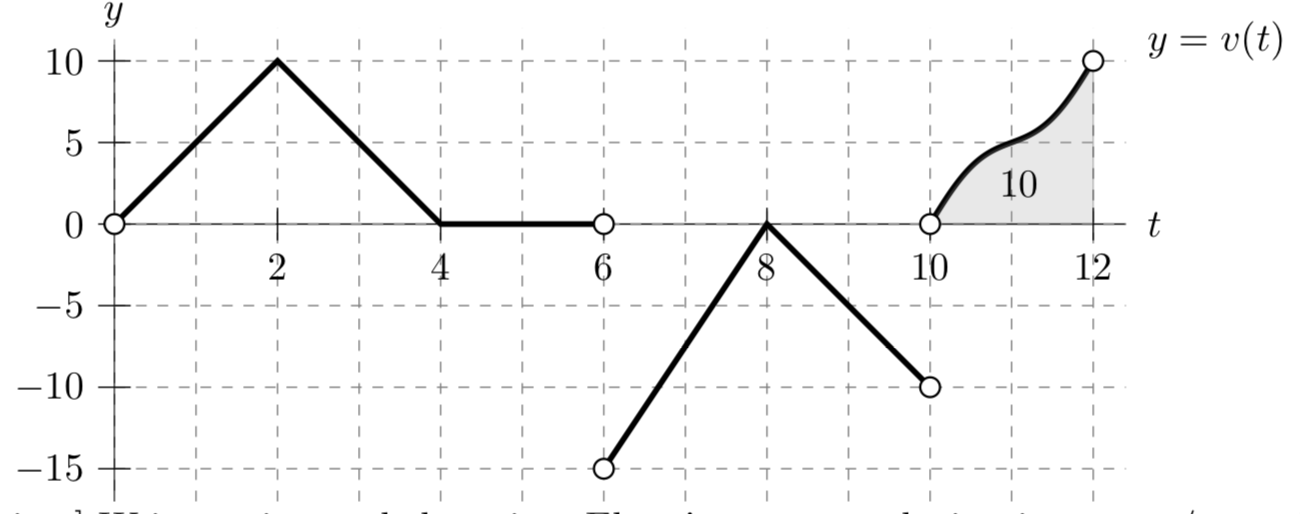
\includegraphics[scale=0.5]{Figures/Elana}
\end{center}
\begin{enumerate}[(a)]
	\item Write an integral that gives Elana's average velocity, in meters/second, from $2$ seconds into the ride until $4$ seconds into the ride. Then compute the exact value of this integral.
	\item Let $h(t)$ be Elana's height (in meters) above the
          ground $t$ seconds after the ride begins. Assume that $h$ is
          continuous, and suppose Elana is at a height of 10 meters
          above the ground when the ride begins. Fill in the exact
          values of \(h(t)\) in the table below.
	$$\begin{array}{|c||c|c|c|c|c|c|c|}
	\hline
	t & 0 & 2 & 4 & 6 & 8 & 10 & 12 \\
	\hline
	h(t) & & & & & & & \\
	\hline
	\end{array}$$
	\item Sketch a detailed graph of $h(t)$ for $0 < t < 12$. In your sketch, be sure that you pay close attention to each of the following:
\begin{multicols}{2}
 \begin{itemize}
 	\item where $h$ is increasing, decreasing, or constant;
 	\item  the values of $h(t)$ you found above;
 	\item where h is/is not differentiable;
 	\item the concavity of the graph of $y = h(t)$.
 \end{itemize}
 \end{multicols}
 \begin{solution}
   See \href{https://dhsp.math.lsa.umich.edu/exams/115exam3/w16/s4.pdf}{https://dhsp.math.lsa.umich.edu/exams/115exam3/w16/s4.pdf}
 \end{solution}
\end{enumerate}
\question (Fall 2017 Final Exam) % problem 1
	The graph of a portion of a function $y = h(x)$ is shown below. Note that the graph is linear where it appears to be linear, including on the intervals $[7, 8]$ and $[10, 11)$.
        \vspace{-0.8cm}
        \begin{center}
          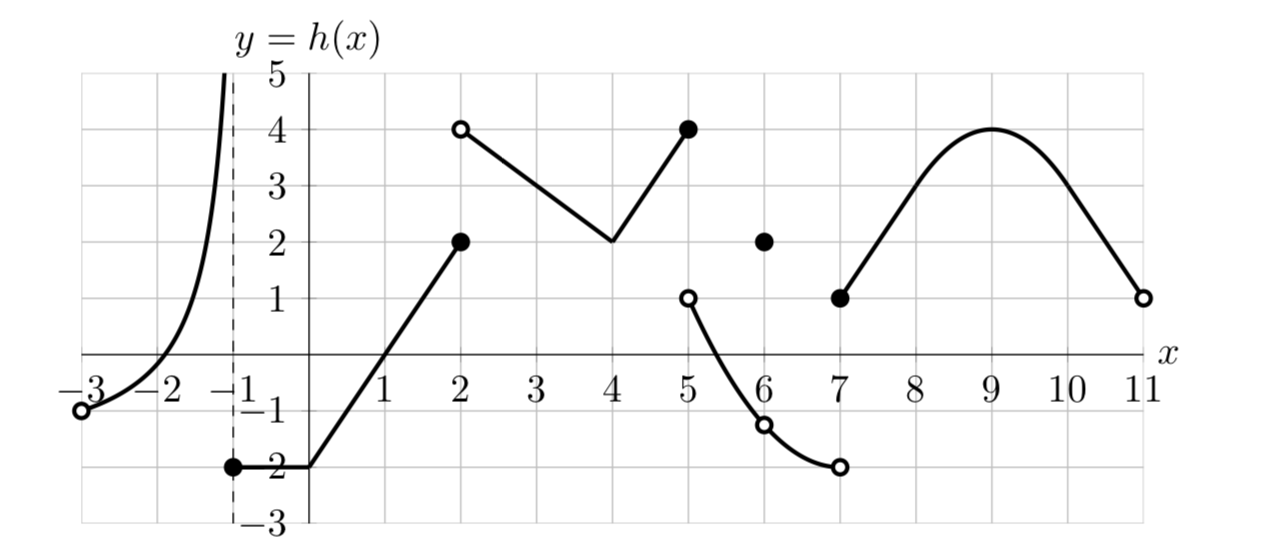
\includegraphics[scale=0.5]{Figures/graph4.png}
        \end{center}
        \vspace{-0.4cm}
\begin{parts}
\part Calculate the average value of \(h(x)\) on \([-1,1]\).
\part Calculate $\displaystyle\int_{7.5}^{10.5} h''(x)$.
\end{parts}
\begin{solution}
  See \href{https://dhsp.math.lsa.umich.edu/exams/115exam3/f17/s1.pdf}{https://dhsp.math.lsa.umich.edu/exams/115exam3/f17/s1.pdf}
\end{solution}
\pagebreak
\question Are the following statements true for all continuous function $f(x)$ and $g(x)$? Give an explanation for you answer (e.g. reference any property of integrals that you may be using). 
\begin{enumerate}[(a)]
\item If $\int_{0}^2 (f(x)+g(x))dx = 10$ and $\int_{0}^2 f(x) dx = 3$, then $\int_{0}^2 g(x) dx$ = 7. 
\item If $\int_{0}^2 f(x) dx = 2$, then $\int_{0}^4 f(x) dx$ = 4. 
\item If $\int_0^2 f(x) dx = 6 $ and $g(x) = 2 f(x)$, then $\int_0^2 g(x) dx = 12$.
\item If $a=b$, then $\int_{a}^{b}f(x) dx = 0$. 
\item $\int_1^2 f(x)dx + \int_2^3 g(x) dx = \int_1^3 (f(x) + g(x)) dx.$  
\item If $f(x) \leq g(x)$ on the inteval $[a,b]$, then the average value of $f$ is less than or equal to the average value of $g$ on the interval $[a,b]$. 
\item The average value of $f$ on the interval $[0,10]$ is the average value of $f$ on $[0,5]$ and the average value of $f$ on $[5,10]$. 
\end{enumerate}
\begin{solution}
  \begin{enumerate}
  \item[(a)] True by linearity of the definite integral.
  \item[(b)] False since \(\int_2^4 f(x) dx\) could be
    anything. (For example, consider \(f(x) = x\)). 
  \item[(c)] True since we can take constant multiples outside of the
    definite integral.
  \item[(d)] True by the Fundamental Theorem of Calculus.
  \item[(e)] False
  \item[(f)] True, since \(\int_a^b f(x) dx \leq \int_a^b g(x) dx\) by
    the comparison property.
  \item[(g)] False. 
  \end{enumerate}
\end{solution}
\question (Fall 2015 Final Exam)
Recall that a function \(h\) is odd if \(h(-x) = -h(x)\) for all \(x\). A portion of the graph
of \(p(x)\), an odd function, is shown below. Assume that the areas of the two shaded regions are
20 and 11, as indicated on the graph, and note that \(p(x)\) is linear for \(16 < x < 20\).
\begin{center}
  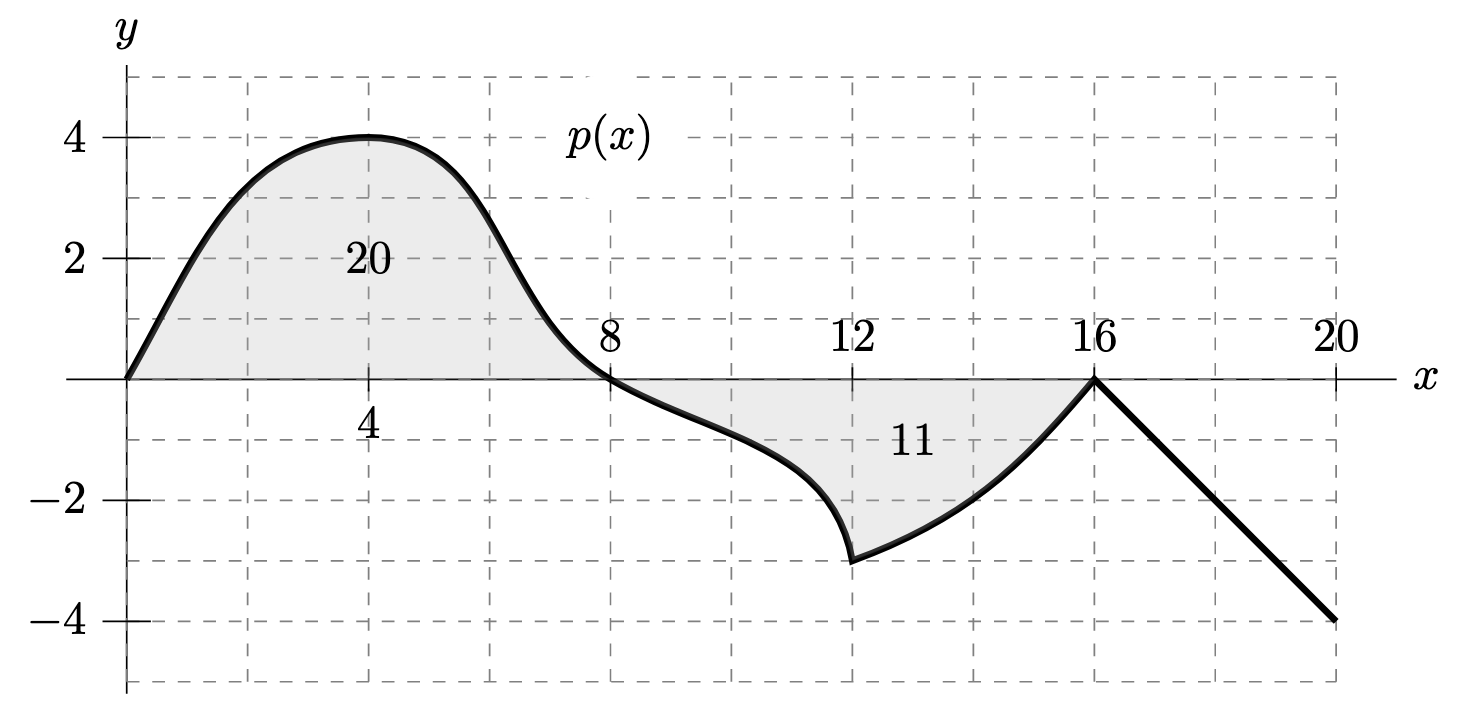
\includegraphics[scale=0.5]{Figures/graph_f15}
\end{center}
\begin{parts}
\part Compute the exact value of \(\int_{0}^{20} (5-3p(x)) dx\).
\part Compute the exact value of \(\int_{4}^8 p'(x) dx\).
\part Find the average value of \(p(x)\) on the interval \(-16 \leq x \leq
  8\).
\part Use a right Riemann sum with 3 equal subintervals to estimate
  \(\int_{12}^{18} p(x) dx\). Write out all terms of the sum.
\end{parts}
\begin{solution}
  See \href{https://dhsp.math.lsa.umich.edu/exams/115exam3/f15/s1.pdf}{https://dhsp.math.lsa.umich.edu/exams/115exam3/f15/s1.pdf}
\end{solution}
\pagebreak
\question Compute the following integrals.
  \begin{enumerate}[(a)]
\item If $f(x)$ is even and $\int_{-2}^{2} ( f(x) - 3) dx = 8$, find $\int_{0}^2 f(x) dx$. 
\item Without any computation, find $\int_{-\pi/4}^{\pi/4} x^3 \cos( x^2 ) dx$. 
  \end{enumerate}
\question (Winter 2019 Final Exam) 

  \begin{minipage}{0.5\linewidth}
    Students from two rival universities had a competition to see who
    could clean up the most litter at a nature preserve.

    University A went first, cleaning up litter from noon to 4pm. Each
    student from University A cleaned at a rate of 12 pounds of litter
    per hour.

    
    Then University B cleaned up litter from 4pm to 8pm.  Each student
    from University B cleaned at a rate of 9 pounds of litter per
    hour.

    Let \(S(t)\) be the number of students cleaning up litter at time
    t hours past noon. The graph of \(S(t)\) is shown to the right.
  \end{minipage}
  \begin{minipage}{0.5\linewidth}
    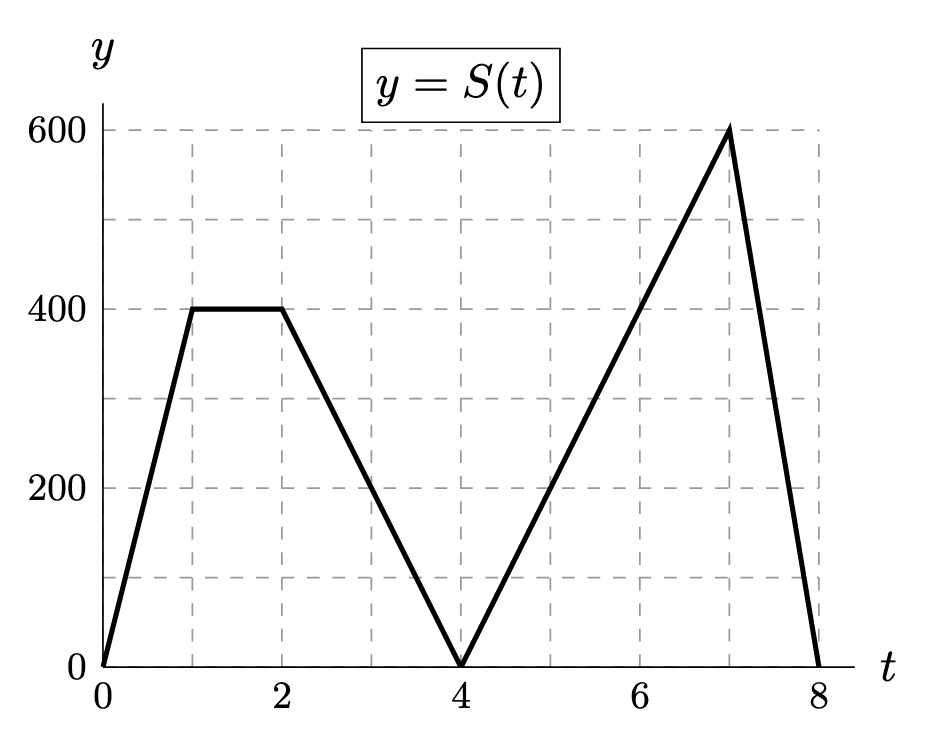
\includegraphics[scale=0.5]{Figures/graph_w19}
  \end{minipage}
  \begin{parts}
  \part Find the total amount of litter cleaned up by University A. Show your work.
  \part Find the total amount of litter cleaned up throughout the entire eight-hour competition. Show your work.
  \part The competition was broadcast live on TV. The number of people viewing the TV

    broadcast at time \(t\) hours past noon is given by the function \[
      B(t) = 4S(t)+200
    \]
    Find the average number of people viewing the TV broadcast during
    the eight-hour competition.
  \end{parts}
  \begin{solution}
    See \href{https://dhsp.math.lsa.umich.edu/exams/115exam3/f19/s9.pdf}{https://dhsp.math.lsa.umich.edu/exams/115exam3/f19/s9.pdf}
  \end{solution}
  \question (Fall 2019 Final Exam)
Given below is a table of values for a function \(g(x)\) and its derivative \(g'(x)\). The functions
\(g(x)\), \(g'(x)\), and \(g''(x)\) are all defined and continuous for all real numbers.
\vspace{-0.5cm}
\begin{center}
  \begin{tabular}{|c|c|c|c|c|c|c|c|c|}
    \hline
    \(x\)&-3&-2&0&2&3&4&6&8\\
    \hline
    \(g(x)\)&2&3&7&9&5&1&-5&-7\\
    \hline
    \(g'(x)\)&0&4&1&0&-2&-4&-1&-3\\
    \hline
  \end{tabular}
\end{center}
Assume that between consecutive values of x given in the table above, g(x) is either always increasing or always decreasing.
Find the quantities in a.–c. exactly, or write nei if there is not enough information provided to do
so.
\begin{multicols}{3}
  \begin{parts}
  \part \(\int_3^6 g(x) dx\)
  \part \(\int_{-2}^2 3g'(x) dx\)
  \part \(\int_0^4 (g''(x)+x) dx\)
  \end{parts}
\end{multicols}
\begin{enumerate}
\item[(d)] Use a right-hand Riemann sum with three equal subdivisions to
  estimate \(\int_2^8 g(x) dx\). Write out all the terms in your
  sum. Is this an underestimate or overestimate?
\end{enumerate}
\begin{solution}
  See \href{https://dhsp.math.lsa.umich.edu/exams/115exam3/f19/s8.pdf}{https://dhsp.math.lsa.umich.edu/exams/115exam3/f19/s8.pdf}
\end{solution}
\end{questions}
\end{document}
%%% Local Variables:
%%% mode: latex
%%% TeX-master: t
%%% End:
